\documentclass[11pt]{article}
\usepackage{amsmath,amsfonts,amsthm,amssymb}
\usepackage{fancyhdr}
\usepackage{extramarks}
\usepackage{chngpage}
\usepackage{graphicx}
\usepackage{algorithm}
\usepackage{algorithmic}
\usepackage{dsfont}
\usepackage{hyperref}
\usepackage{enumerate}
\usepackage{color}
\usepackage{datetime}
\usepackage{booktabs}

\newdateformat{monthyeardate}{\monthname[\THEMONTH], \THEYEAR}

\newtheorem{theorem}{Theorem}
\newtheorem{lemma}{Lemma}

\renewcommand{\algorithmicrequire}{\textbf{Input:}}
\renewcommand{\algorithmicensure}{\textbf{Output:}}

% In case you need to adjust margins:
\topmargin=-0.3in      %
\oddsidemargin=0.25in      %
\textwidth=6in        %
\textheight=8.5in       %
\headsep=0.25in         %

\linespread{1.1}

% Setup the header and footer
\pagestyle{fancy}                                                       %
\lhead{}                                                 %
\chead{}  %
\rhead{\firstxmark}                                                     %
\lfoot{\lastxmark}                                                      %
\cfoot{}                                                                %
\rfoot{Page\ \thepage}                          %
\renewcommand\headrulewidth{0.4pt}                                      %
\renewcommand\footrulewidth{0.4pt}                                      %

%%%%%%%%%%%%%%%%%%%%%%%%%%%%%%%%%%%%%%%%%%%%%%%%%%%%%%%%%%%%%
% Make title
\title{\textsc{Computational Biology}\\ \vspace{0.06in}{\bf\Large Project 1: Automated Particle Picking in Cryo-EM}}
\author{\vspace{0.05in}\textbf{An Ju \qquad Yangkun Zhang \qquad Tianxiao Shen}\\Institute for Interdisciplinary Information Sciences}
\date{\monthyeardate\today}
%%%%%%%%%%%%%%%%%%%%%%%%%%%%%%%%%%%%%%%%%%%%%%%%%%%%%%%%%%%%%

\begin{document}
\maketitle \thispagestyle{empty}

%%%%%%%%%%%%%%%%%%%%%%%%%%%%%%%%%%%%%%%%%%%%%%%%%%%%%%%%%%%%%
% Begin edit from here

\section{Introduction}
This project is to pick particles from micrograph in cryo-electron microscopy (cryo-EM) \cite{liao2013structure}. Given a micrograph, our system will predict the center coordinates of particles in it.

We address this problem in a two-step procedure: first, we scan the whole micrograph by a sliding window and judge whether it contains a particle or not \cite{langlois2014automated}; and then, for all the windows containing a particle, we compute their center and merge the ones nearby to get the final results.

An Ju programmed the major part. Yangkun Zhang assisted in coding and did program optimization, including efficient GPU implementation. Tianxiao Shen was in charge of algorithm design, report and demo. We did experiments and analysis together.

\section{Algorithm}
\subsection{Window Classification}
To judge whether a window contains a particle or not is a binary classification problem. We use a convolutional neural network (CNN) to deal with this task, which is one of the most powerful machine learning algorithms for image classification \cite{krizhevsky2012imagenet} .

\subsubsection{Preprocessing}
We preprocess all the values to make them range between 0 and 1, by subtracting $\min$ and then dividing by $\max-\min$. We directly train our network on these values.

\subsubsection{Network Architecture}
Our network contains 5 learned layers---3 convolutional and 2 fully-connected. The convolutional layers have 48 kernels of size $11\times11$ with stride 4, 128 kernels of size $5\times5$ with stride 1, and 197 kernels of size $3\times3$ with stride 1 respectively. Each of them is followed by a max-pooling layer. The first fully-connected layer has 512 neurons, and the second has 2 neurons, corresponding to the two classes.

We use Rectified Linear Units (ReLUs) nonlinearity, and the final layer is fed to a 2-way softmax to produce a Bernoulli distribution. We use the cross-entropy between the true and predicted distribution as our loss function. And we use Stochastic Gradient Descent (SGD) with Nesterov momentum to train our model \cite{sutskever2013importance}. Each micrograph is a batch.

\subsubsection{Training Data}
As the two classes are skewed---most windows do not contain a particle, we adopt a simple strategy to get balanced training data: all golden particles are used as positive cases (each particle determines a window by locating its center), and we randomly sample negative cases of the same amount.

\subsection{Merge Neighboring Windows}
A particle could be contained by multiple overlapping windows, and thus we need to merge them into a single one. For a window predicted to have a particle in it, we compute the coordinates of its center and find its nearest neighbor among all the particles picked so far. If the distance between them is less than a threshold $d$, we merge them in the center of mass way; otherwise we regard it as a new particle.

We calculate the confidence of a particle by summing up its components' confidence minus 0.5, since 0.5 is the bias. If this value is greater than a threshold $C$, we report it as a final predicted particle.

The overall procedure is described in Algorithm \ref{merge}.

\begin{algorithm}[htbp]
\caption{Particle Picking}\label{merge}
\begin{algorithmic}[1]
\REQUIRE a micrograph $g$
\ENSURE a list $l$ of particles
\STATE $l,\hat l\leftarrow\emptyset$

\FORALL {window $w$ in $g$}
    \STATE $(p_0, p_1)\leftarrow$ CNN$(w)$
    \IF {$p_1>0.5$}
        \STATE $(x_w,y_w)\leftarrow$ center$(w)$
        \STATE $(x,y,m,c)\leftarrow$ findNearestNeighbor$((x_w,y_w),\hat l)$
        \IF {dist$\left((x_w,y_w),(x,y)\right)<d$}
            \STATE $(x,y)\leftarrow (\frac{mx+x_w}{m+1}, \frac{my+y_w}{m+1})$
            \STATE $(m,c)\leftarrow (m+1,c+p_1-0.5)$
        \ELSE
            \STATE $\hat l\leftarrow \hat l\cup\{(x_w,y_w,1,p_1-0.5)\}$
        \ENDIF
    \ENDIF
\ENDFOR

\FORALL {$(x,y,m,c) \in \hat l$}
    \IF {$c > C$}
        \STATE $l\leftarrow l\cup\{(x,y)\}$
    \ENDIF
\ENDFOR
\end{algorithmic}
\end{algorithm}

\section{Experiments}
There are 40 micrographs in training data, from which we use 32 to train our network, and 8 for validation to tune the hyper-parameters. The results are based on 20 blind testing micrographs.

\subsection{Parameters Setting}
The window size is $200\times 200$, and the stride is 15. Distance threshold $d=30$. Confidence threshold $C=1.65$. 

\subsection{Results}
For window classification, our model achieves 93.54\% accuracy. Table \ref{performance} shows the performance on test data. The average precision, recall, and F-measure are 59.33\%, 74.26\%, 64.46\% respectively.

\begin{table}[htbp]
\begin{center}
\begin{tabular}{lcccccccccc}
\toprule
Index & 1 & 2 & 3 & 4 & 5 & 6 & 7 & 8 & 9 & 10\\
\hline
Precision & 64.96 &	57.19 &	67.77 &	53.33 &	49.47 &	70.00 &	72.00 &	66.94 &	60.53 &	23.25\\
Recall    & 83.33 &	96.62 &	86.42 &	71.15 &	86.96 &	56.44 &	64.29 &	42.94 &	85.21 &	70.89\\
F-measure & 73.01 &	71.85 &	75.97 &	60.97 &	63.06 &	62.49 &	67.92 &	52.32 &	70.78 &	35.01\\
\toprule
Index & 11 & 12 & 13 & 14 & 15 & 16 & 17 & 18 & 19 & 20\\
\hline
Precision & 58.30 &	69.48 &	58.42 &	57.84 &	59.80 &	74.74 &	71.74 &	23.59 &	58.21 &	69.09\\
Recall    & 87.65 &	87.76 &	84.66 &	73.76 &	85.55 &	69.89 &	54.34 &	38.60 &	84.38 &	74.47\\
F-measure & 70.03 &	77.56 &	69.13 &	64.84 &	70.39 &	72.24 &	61.84 &	29.28 &	68.89 &	71.68\\
\toprule
\end{tabular}
\end{center}
\caption{Precision, recall, and F-measure on test data.}\label{performance}
\end{table}

\section{Discussion}

\subsection{Contaminant}
Our model performs poorly on micrograph 10 and 18. We find that they have a large area of contaminants, which lead to numerous false positives (see figure \ref{contaminant}).

Follow \cite{langlois2014automated}, we tried to do Principal Component Analysis (PCA) over the power spectra of extracted windows, and eliminate outliers according to their distribution. But it did not work :(. We think a procedure of edge detection, connected components labeling and convex hull computation \cite{zhu2004contaminant} might be a good solution to detect contaminants.

\begin{figure}[htbp]
\centering
    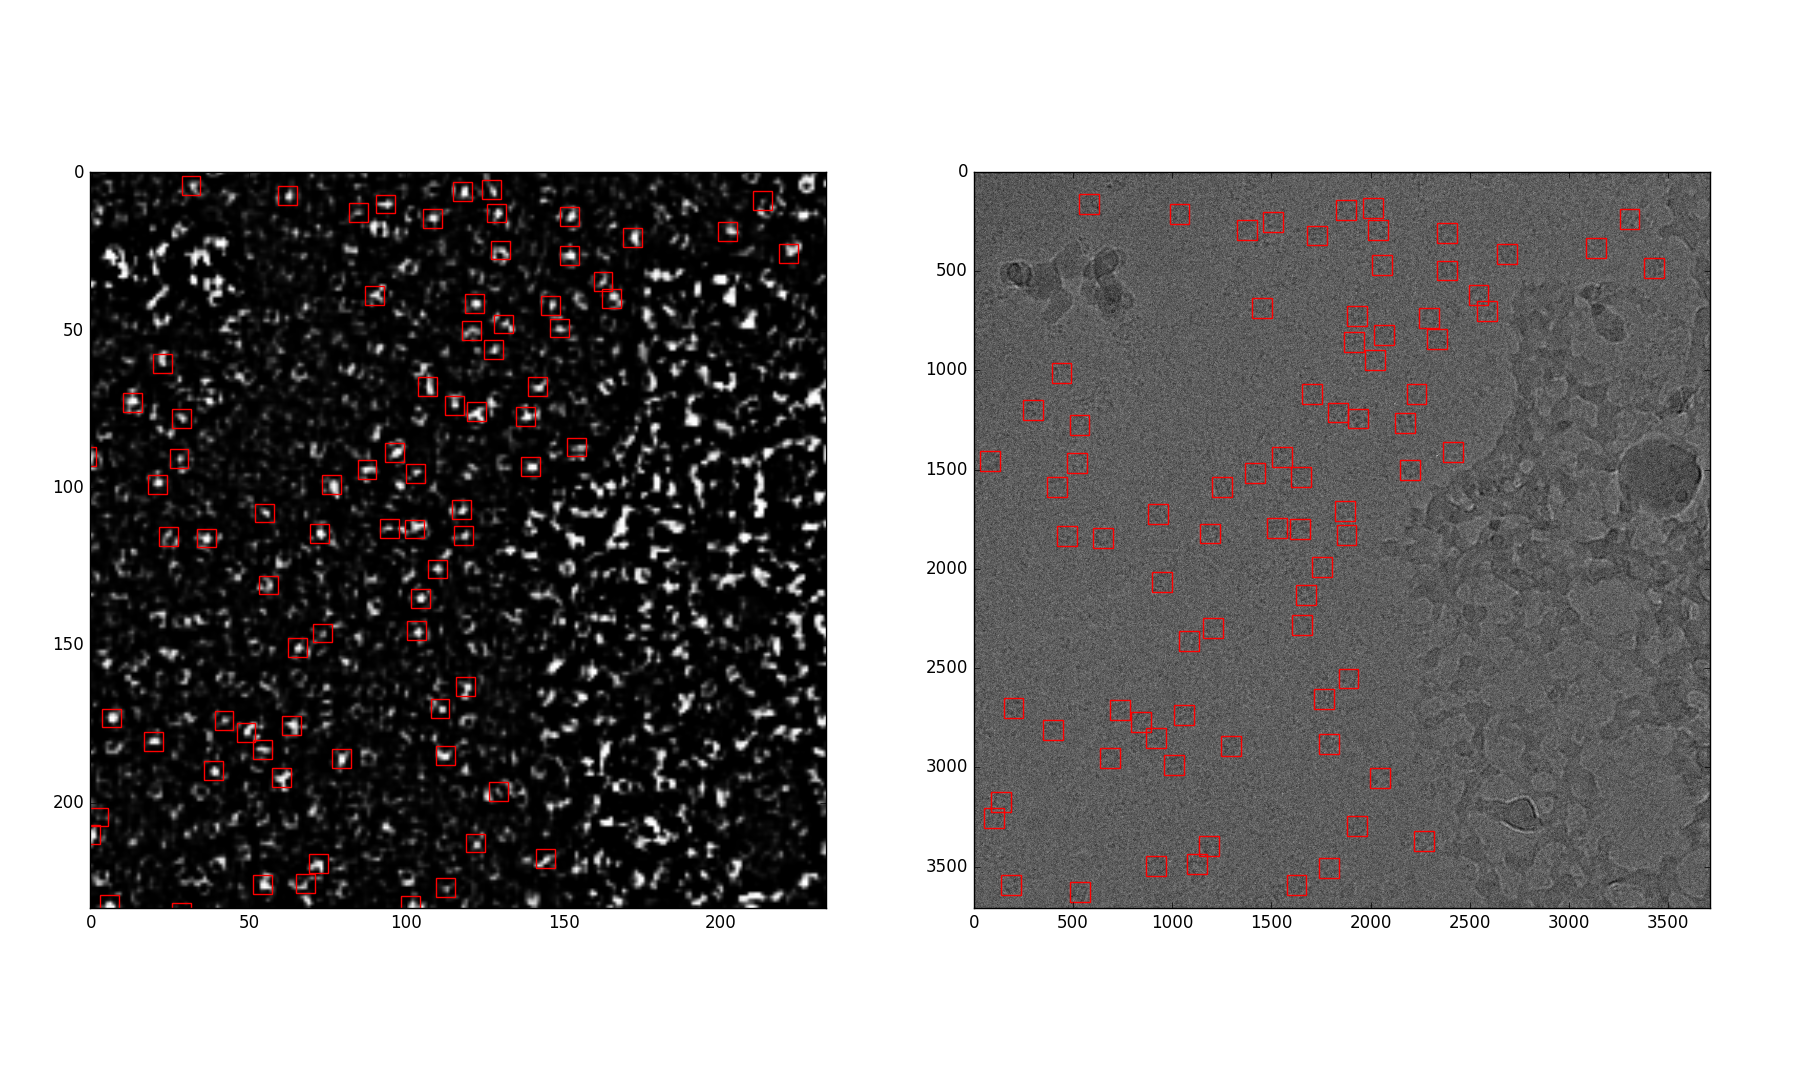
\includegraphics[width=0.8\textwidth]{figure_test9.png}
    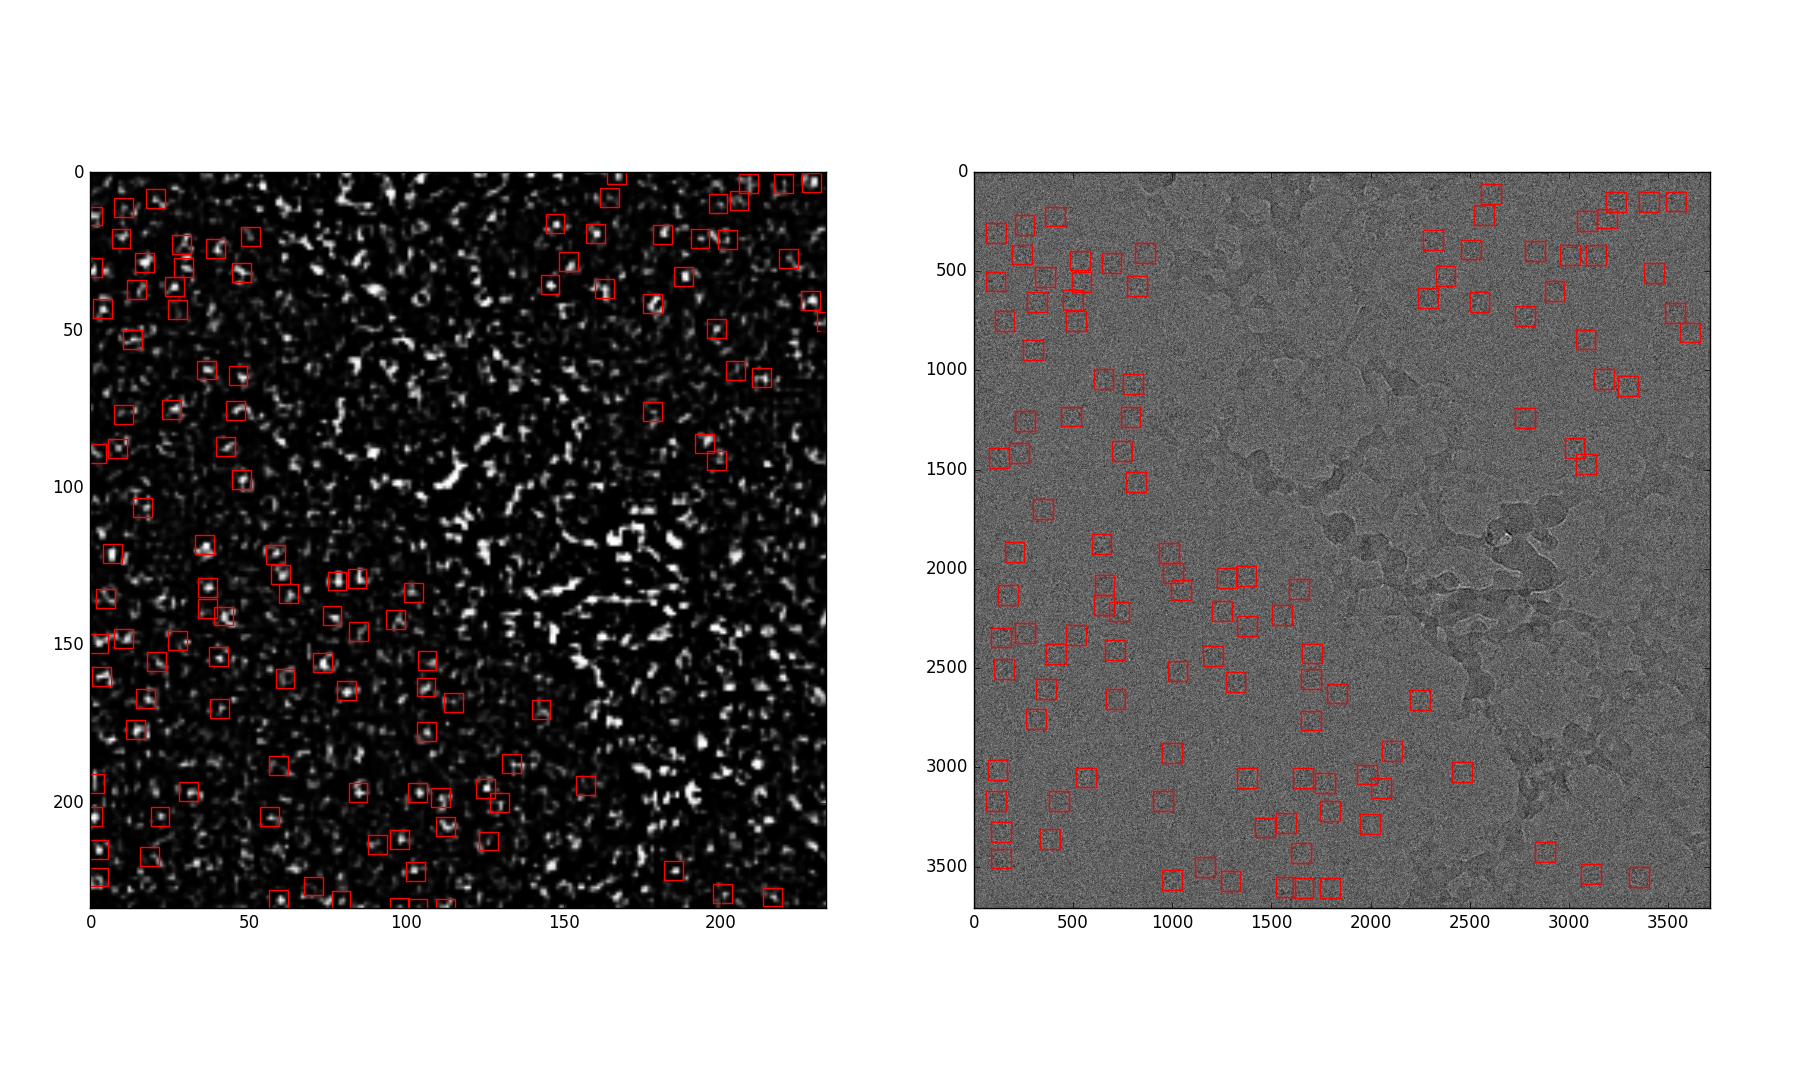
\includegraphics[width=0.8\textwidth]{figure_test17.png}
\caption{Micrograph 10 and 18 in test data. Images on the left show our network's output confidence (probability of containing a particle). Images on the right are original micrographs. Red windows contain golden particles as their center.}\label{contaminant}
\end{figure}

\subsection{Boundary}
When we tested on validation data, we realized that we did not consider windows lying out. Therefore, we failed to pick out particles on the boundary (see figure \ref{boundary}).

We tried various padding methods to take these incomplete windows into consideration, including padding with mean, Gaussian noise, and folding. But none of them worked :(. Nevertheless, it seems that these particles do not affect evaluation much.

\begin{figure}[htbp]
\centering
    \includegraphics[width=0.7\textwidth]{figure_train40.png}
\caption{Micrograph 8 in validation data (i.e. micrograph 40 in all training data). Green points are predicted particles. Red windows contain golden particles as their center. On the bottom there are several windows lying out, which we missed.}\label{boundary}
\end{figure}

\section*{Acknowledgments}
We thank Zhipeng Jia for the helpful discussion with him.

% End edit to here
%%%%%%%%%%%%%%%%%%%%%%%%%%%%%%%%%%%%%%%%%%%%%%%%%%%%%%%%%%%%%

\bibliographystyle{abbrv}
\bibliography{bibfile}

\end{document}

%%%%%%%%%%%%%%%%%%%%%%%%%%%%%%%%%%%%%%%%%%%%%%%%%%%%%%%%%%%%%
